%This template is based on one provided by the American Physical Society for submission to its journals.

\documentclass[aps,twocolumn,showpacs,preprintnumbers]{revtex4}

%The following packages add LaTeX commands that make formatting and writing math easier

\usepackage{graphicx}  % Include figure files
\usepackage{subfigure}
\usepackage{multirow}
\usepackage{verbatim}

\linespread{1.1}
\usepackage{fancyhdr}
\usepackage{longtable}
\usepackage{parskip}
\usepackage[T1]{fontenc}
\usepackage{dcolumn}   % Align table columns on decimal point

\usepackage{bm}        % bold math
\usepackage{amsfonts}  % Common math fonts
\usepackage{amsmath}   % Common math functions
\usepackage{amssymb}   % Common math symbols

%The following custom commands simplify commonly used LaTeX commands

\newcommand{\pic}[2]{\begin{center} \includegraphics[scale=#1]{#2}\end{center}}
\newcommand{\re}[1]{\mathrm{Re}\left(#1\right)}
\newcommand{\im}[1]{\mathrm{Im}\left(#1\right)}
\newcommand{\bdot}[1]{\dot{ \bb {#1}}}
\newcommand{\bddot}[1]{\ddot{ \bb {#1}}}
\newcommand{\bidot}[1]{\dot{ \bi{ #1}}}
\newcommand{\biddot}[1]{\ddot{ \bi {#1}}}
\newcommand{\ep}{\varepsilon}
\newcommand{\for}{\quad \quad \mathrm{for} \quad\quad}
\newcommand{\then}{\quad \quad \implies \quad\quad}
\newcommand{\an}{\quad \quad \mathrm{and} \quad\quad}
\newcommand{\ifff}{\quad \quad \mathrm{if} \quad\quad}
\newcommand{\where}{\quad \quad \mathrm{where} \quad\quad}
\newcommand{\dg}{^\dagger}
\newcommand{\semi}{\quad \quad \mathrm{;} \quad\quad}
\newcommand{\paren}[1]{\left( #1 \right)}
\newcommand{\brac}[1]{\left[ #1 \right]}
\newcommand{\bra}[1]{\left\langle #1 \right|}
\newcommand{\exv}[1]{\left\langle #1 \right\rangle}
\newcommand{\pwisein}{\left\{ \begin{array}{ll}}
\newcommand{\pwiseout}{\end{array}\right.}
\newcommand{\ket}[1]{\left| #1 \right\rangle}
\newcommand{\bracket}[2]{\left\langle #1 | #2 \right\rangle}
\newcommand{\trace}[1]{\mathrm{Tr} \left( #1 \right)}
\renewcommand{\det}[1]{\mathrm{det}\left( #1 \right)}
\newcommand{\del}[1]{\frac{\partial}{\partial #1}}
\newcommand{\fulld}[1]{\frac{d}{d #1}}
\newcommand{\fulldd}[2]{\frac{d #1}{d #2}}
\newcommand{\dell}[2]{\frac{\partial #1}{\partial #2}}
\newcommand{\delltwo}[2]{\frac{\partial^2 #1}{\partial #2 ^2}}
\newcommand{\bb}{\mathbf}
\newcommand{\bi}{\boldsymbol}
\newcommand{\eq}[1]{\begin{equation} #1 \end{equation}}
\newcommand{\radhalf}{ \frac{ \sqrt{2}}{2}}
\newcommand{\sigx}{\left( \begin{array}{cc} 0 & 1\\ 1 & 0 \end{array}\right)}
\newcommand{\sigy}{\left( \begin{array}{cc} 0 & -i\\ i & 0 \end{array}\right)}
\newcommand{\sigz}{\left( \begin{array}{cc} 1 & 0\\ 0 & -1 \end{array}\right)}
\renewcommand{\matrix}[1]{\left( \begin{array} #1 \end{array}\right)}
\newcommand{\thermo}[3]{\left( \frac{\partial #1}{\partial #2} \right)_{#3}}
\newcommand{\coolfrac}[2]{\left( \frac{ #1}{ #2} \right)}

\setlength{\parindent}{10pt}

\begin{document}

\title{Gravity Tunnel through the Earth using  an effective mass density function}

\author{Nicolás Gómez, Carlos Quimbay}

\affiliation {\it Departamento de Física, Universidad Nacional de Colombia, Bogotá D.C., Colombia}

\date{\today}

\begin{abstract}  

%FIRST ATTEMPT
%The gravity tunnel problem is faced with the use of a decreasing power law function as the mass density. Some parameters are introduced and determined to find a concordance between the traversal times found using the density profile from seismic data and the power law function. A trustworthy concordance is found in traversal times, velocity profiles and shapes of the braquistochrones , making our proposition an effective mass density function that can describe the interior of the Earth.

%SECOND ATTEMPT

A novel effective function for the mass density profile inside the Earth is proposed in order to describe qualitatively and quantitatively physical aspects of the terrestrial density proposed by seismic models within the context of the gravity tunnel. This was done using a decreasing potential law function dependent only on the distance to the center of the Earth and on some parameters, in such a way that gravity on the surface and total mass are correctly predicted, and that the disagreement of the traversal times of a gravity train with those obtained by the seismic data are minimum.  To do this we first determined the first parameter to obtain a family of density functions whose integrals give us the right $g$ constant and mass of the Earth, then we analytically computed the velocities and used them to let a program minimize the relative traversal times function, and finally we used those results to calculate chord path times, braquistochrones shapes and braquistochrones paths and compared them with those of the model, finding a high correspondence.





\end{abstract}


\maketitle 

\section{Introduction}

%P1: Intro: scientific motivation
    Un túnel gravitacional es un medio de transporte hipotético en el que, para llegar de un punto a otro en la superficie del planeta, se recurre a la aceleración de la gravedad en un túnel conectando ambos puntos. El problema es netamente pedagógico y ha sido discutido ampliamente en revistas de este carácter
    \citep{History-Tunels}. 
%P2: More intro: approach, definitions, history, context, rationale    
    
     Esto ha sido realizado de múltiples maneras, considerando el caso más sencillo de densidad constante\citep{Venezian}, propuesto como ejercicio en libros de texto de mecánica \cite{Goldstein}, adicionándole la fricción del riel \citep{Tunel-friccioon}, o considerando la rotación de la Tierra \citep{Solomon2, Iserman2, Simonic}, y el efecto de ésta en su forma\citep{Taillet2018},  o incluso en el marco de la relatividad general \citep{Parker2017, Seel}.   De igual manera se han visto trabajos considerando relaciones de densidad-presión basados en politropas \citep{Tunel-Potencia, Politropes2}, o en modelos geofísicos con densidades más realistas como el llamado modelo de referencia preliminar de la Tierra (PREM), siendo este hecho numéricamente por Klotz \citep{gravity-train-prem}, haciendo una comparación  con una aproximación de gravedad constante, y también haciendo un tratamiento analítico usando una aproximación lineal que arroja resultados más cercanos con el modelo de referencia preliminar de la Tierra y que se libra de la poco físicamente realista situación de una gravedad constante (dado que eso implica densidades infinitas en el centro del planeta).\citep{gravity-train-prem-approx, Iserman2}. 

    Tanto para fines geofísicos, astrofísicos como puramente físicos, conocer la distribución de la densidad en nuestro planeta es de gran utilidad. En primera aproximación y para fines netamente ilustrativos se puede tomar constante, dividiendo la masa total entre su volumen, obteniendo $\Bar{\rho}=5515kg/m^3$\citep{AstronomicalConstants}.  Con esto se pueden obtener valores aproximados para la aceleración gravitacional o momentos de inercia. Sin embargo, es claro que la densidad de la Tierra (y de cualquier cuerpo astronómico) dista mucho de ser constante. Otros modelos se han propuesto para describir la densidad \citep{Snyder1985} o la aceleración \citep{Dragoni2020} de 
    la Tierra, pero el modelo más aceptado es el modelo de referencia preliminar, según el cual la densidad en el interior de nuestro planeta tiene discontinuidades entre las diferentes capas que la componen: núcleo interno, núcleo externo, manto, corteza y superficie (océano). Dentro de cada región la densidad se aproxima con una función polinomial.\citep{PREM} Esto se puede apreciarse en la figura \ref{fig:Prem density}. Como se puede notar, la densidad aumenta hacia el centro y alcanza un valor máximo de alredor de $13000kg/m^3$, mientras que en la superficie es casi $1000kg/m^3$, que corresponde a la densidad del agua en el océano. 
    
    A pesar de los múltiples datos que fueron necesarios para establecer dicho modelo, no deja de ser una abstracción matemática. En el presente trabajo se pretende discutir una posible aproximación a este modelo usando una función de densidad efectiva matemáticamente más sencilla de expresar; suave, continua y ciertamente no constante. Esta función se plantea como un posible reemplazo a la descrita por el modelo de referencia y por lo tanto como una descripción sencilla pero acertada en sus efectos.
    
    Específicamente se usan dos perfiles,dados por funciones decrecientes como ley de potencia, estableciendo dos y tres parámtros, entre ellos la potencia misma, para obtener de ella la mayor física posible. Es decir, se busca que el perfil de densidad efectiva dé cuenta de la masa total de la Tierra, de que la aceleración gravitacional en la superficie es $g=9.81 m/s^2$ y que los tiempos de caída en un túnel gravitacional coincidan lo mejor posible con los del modelo PREM. Esto, con el fin de que el perfil densidad efectiva se muestre como una confiable y simple descripción del interior de la Tierra.
    
    El uso de esta función no solo representa un tratamiento completamente diferente a los que se han mencionado para el problema del túnel gravitacional, sino que sirve como ejemplo para ilustrar la construcción y el desarrollo de una teoría o modelo efectivo. Modelos efectivos en mecánica clásica y en general en física de nivel de pregrado son escasos, sin embargo su utilidad en el mundo científico es cada vez mayor, razón por la cual es importante que estudiantes de una carrera de física o ingeniería se familiaricen con alguno que contenga una física sencilla y que no requiera de métodos matemáticos o computacionales muy elaborados. El presente artículo cumple con todos estos requisitos, ya que las deducciones se presentan en el marco de la mecánica de Newton y las funciones usadas son todas integrables ya sea en términos de funciones igualmente sencillas, o numéricamente usando los métodos convencionales. 
    
%P3: What you did, what you found 

    Para abordar el probelma del tunelamineto gravitacional, se plantean primero los posibles perfiles de densidad en la sección \ref{density section}, se deducen las funciones de aceleración, y en la sección \ref{velocity section}, se discute sobre los perfiles de velocidad. En \ref{time section} se hallan las expresiones para los tiempos de tunelamiento dependientes de la densidad y se minimizan las funciones pertinentes para que los tiempos se aproximen como se requiere. Posteriormente calculamos dichos tiempos y comparamos los resultados obtenidos con los parámetros que resultan de la minimización tanto en las velocidades y los tiempos de tunelamiento, como en la forma de las trayectorias braquistócrona (\ref{braquistochrone section}) y sus respectivos tiempos.
    
    Finalmente, en \ref{acceleration section} estudiamos la aceleración a lo largo del camino, esto para dar una explicación dinámica del por qué los tiempos son menores para caminos más largos como las braquistócronas, y no para los caminos de menor distancia.
    
    

    \begin{figure}
        \centering
        \includegraphics[scale=0.6]{Figures/prem-profile.pdf}
        \caption{Density on the inside of the Earth as a function of the radius according to the data obtained by PREM.}
        \label{fig:Prem density}
    \end{figure}




    
\section{Density Profile}\label{density section}

    Para dar cuenta de una densidad que reemplace a la de la figura \ref{fig:Prem density}, buscamos, no extactamente describir la misma situación de la distribución de masa de manera local, sino reproducir sus efectos. Partamos para ello de la forma de densidad potencial más sencilla, dada por
    
    \begin{equation}
        \rho(r) = \Bar{\rho} \left( \frac{R-r}{R}\right)^b,
        \label{densidad general}
    \end{equation}
    con $\Bar{\rho} = 3M/4 \pi R^3$ la densidad promedio de la Tierra, y $b$ una potencia real positiva. Con esta densidad, se obtiene la aceleración de la gravedad, a partir de la ley de Gauss y usando el teorema del binomio de Newton
    
    \begin{align*}
          a (r) &= \frac{4 \pi G}{r^2}  \int_0^r \rho (r') {r'}^2 dr' \\
          %&=  \frac{4 \pi G}{r^2} \frac{3M}{4 \pi R^3} \frac{1}{R^b} \sum_{k=0}^{\infty} \binom{b}{k} R^{b-k} (-1)^k  \int_0^r  {r'}^{k} {r'}^2 dr' \\
          &= \frac{3 GM}{R^2} \sum_{k=0}^{\infty} \binom{b}{k} R^{-(k+1)} (-1)^k \frac{r^{k+1}}{k+3} \\
          &= 3g  \sum_{k=0}^{\infty} \binom{b}{k} (-1)^k R^{-(k+1)}  \frac{r^{k+1}}{k+3} .
    \end{align*}

    Tomemos el caso particular $b=1$ (correspondiente a una función lineal), en la superficie se tendría 
    
    \begin{align*}
        a(R) = \frac{1}{4}g.
    \end{align*}
    
    Vemos que la aceleración de la gravedad en la superficie de la Tierra sería de $g/4$, no $g$. De manera que este perfil no puede ser usado si se pretende que las cantidades medibles en el exterior coincidan con los valores conocidos.
    
    \subsection{Density with two parameters}
    
    Consideremos entonces un cambio sencillo a \eqref{densidad general} dado por
    
     \begin{equation}
        \rho_1(r) = \rho_0 \left( \frac{R-r}{R}\right)^b,
        \label{densidad general modificada}
    \end{equation}
    con $\rho_0 \propto \Bar{\rho}$, pero que al hallar la aceleración se cumpla $a(R) = g$. Con esto, 
    
     \begin{align*}
          a (r) %&= \frac{4 \pi G}{r^2}  \int_0^r \rho (r') {r'}^2 dr' \\
          =  4 \pi G \rho_0  \sum_{k=0}^{\infty} \binom{b}{k} (-1)^k R^{-k}  \frac{r^{k+1}}{k+3}, 
    \end{align*}
    y así, en la superficie se tiene
    
    \begin{align*}
        g &= 4 \pi G \rho_0  \sum_{k=0}^{\infty} \binom{b}{k} (-1)^k  \frac{R}{k+3} \\ 
        &= 4 \pi G \rho_0 R k_1(b),
    \end{align*}
    siendo $k_1(b)$ el coeficiente 
    
    \begin{equation*}
        k_1(b) =  \sum_{k=0}^{\infty} \binom{b}{k}  \frac{(-1)^k }{k+3} ,
    \end{equation*}
    despejando ahora para $\rho_0$,
    
    \begin{align*}
        \rho_0 = \frac{g}{4\pi G k_1(b)} %= \frac{1}{4\pi G c_b} \frac{GM}{R^2}\\
        %&= \frac{1}{3c_b} \left( \frac{3M}{ 4\pi R^3}\right)\\
        = \frac{1}{3k_1(b)} \Bar{\rho},
    \end{align*}
    de esta manera, \eqref{densidad general modificada} queda
    
    \begin{equation}
        \rho_1 (r;b) = \frac{\Bar{\rho}}{ 3 k_1(b)}  \left( \frac{R-r}{R}\right)^b,
        \label{densidad efectiva 1}
    \end{equation}
    y la aceleración en cualquier punto $r<R$ es
    
    \begin{equation}
        a_1 (r;b) = \frac{g}{c_b} \sum_{k=0}^{\infty}  \binom{b}{k} \frac{(-1)^k}{k+3} \left(\frac{r}{R} \right)^{(k+1)}.
        \label{aceleración gravitacional general}
    \end{equation}
 
    
    
    \subsection{Effective density with three parameters:}
    
    Otra posible forma para la densidad sería usando cuatro parámetros, pero se puede reducir a solo tres parámetros
    
    \begin{equation*}
        \rho(r) = N \Bar{\rho} \left( \frac{\alpha R - \beta r}{R}\right)^b = a \Bar{\rho} \left( \frac{ R - c r}{R} \right)^b,
    \end{equation*}
    Este perfil de densidad, no obstante, tiene el problema de que en la superficie, la densidad es distinta de cero, lo cual representa un problema si se quiere describir adecuadamente este aspecto. Una alternativa que cumple el mismo propósito sería 
    
    \begin{equation}
        \rho_2(r) = a \Bar{\rho} \left(  1 - \frac{(1+c) r/R}{1+c \; r/R} \right)^b
        \label{densidad general 2}
    \end{equation}
    con $a,b,c$ a determinar de modo que $a(R)=g$ y que se aproxime a $\rho_{PREM}$ lo mejor posible. Nótese que para esta función si se cumple $\rho_2(R; b, c) = 0$, y además, $\rho_2(r;b,0) = \rho_1 (r;b)$.
    
    El primero de estos parámetros se fija nuevamente con la aceleración. De manera análoga, usando 
    
    
     \begin{align}
          a_2 (r) &= \frac{4 \pi G a  \Bar{\rho} }{r^2} \int_0^r  \left(  1 - \frac{(1+c) r'/R}{1+c \; r'/R} \right)^b r'^2 dr'
          \label{aceleración gravitacional general 2}
    \end{align}
    encontramos que
    
     \begin{align*}
        a =\frac{1}{3k(b,c)},
    \end{align*}
    con el nuevo coeficiente
    
    \begin{equation*}
        k_2(b,c) =   \int_0^R  \left(  1 - \frac{(1+c) r'/R}{1+c \; r'/R} \right)^b r'^2 dr'
    \end{equation*}
   con esto la densidad es
    
    \begin{equation}
         \rho_2(r;b,c) = \frac{\Bar{\rho}}{3k_2(b,c)} \left( 1- c\frac{r}{R}\right)^b.
         \label{densidad efectiva 2}
    \end{equation}
    La aceleración para este caso es 
    
    \begin{equation}
        a_2 (r;b,c) = \frac{g}{k(b,c)} \sum_{k=0}^{\infty} \binom{b}{k} \frac{(-c)^k}{k+3} \left(\frac{r}{R} \right)^{(k+1)}.
        \label{aceleración gravitacional general 2}
    \end{equation}
    
    En la figura \ref{fig:gravity} se puede apreciar la comparación de las aceleraciones según estas funciones analíticas y según los datos numéricos del modelo PREM. Como se puede notar, las funciones son suaves y, aunque no necesariamente se acercan tanto a la aceleración en cada punto $r<R$, toman el mismo valor para $r=R$, i.e., $9.81m/s^2$
    
    
    \begin{figure}
        \centering
        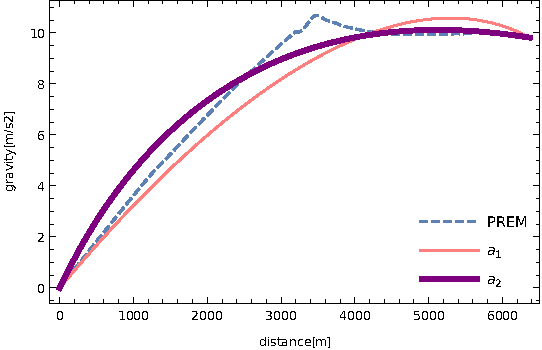
\includegraphics[scale=0.85]{Figures/accelerations.pdf}
        \caption{Acceleration profiles according to PREM data and to \eqref{aceleración gravitacional general} and \eqref{aceleración gravitacional general 2} functions.} 
        \label{fig:gravity}
    \end{figure}
    
    La siguiente condición física que se debe cumplir es que la masa total de la Tierra debe coincidir con el valor de la literatura M. Afortunadamente esto se obtiene directamente de las consideraciones anteriores para la gravedad, dado que la integral es esencialmente la misma y que, de hecho, es la masa total la que da a la aceleración de la gravedad su valor en la superficie: 
    
    \begin{comment}
    \begin{align*}
        \mathcal{M}(R) &= 4 \pi \int_{0}^R \rho(r') {r'}^2 dr' \\
         &= 4 \pi  \frac{\Bar{\rho}}{3k(b,c)} \sum_{k=0}^{\infty} \binom{b}{k} (-c)^k R^{-k}  \frac{r^{k+3}}{k+3} \\
         &=   \frac{4\pi}{3k(b,c)} \left(\frac{3 M}{4\pi R^3} \right) \sum_{k=0}^{\infty} \binom{b}{k} (-c)^k R^{-k}  \frac{R^{k+3}}{k+3} \\
         &= \frac{M}{3k(b,c)} \sum_{k=0}^{\infty} \binom{b}{k} (-c)^k   \frac{1}{k+3} = M.
    \end{align*}
    \end{comment}
    
\section{Determination of the velocity profile}\label{velocity section}
    
       Una vez conocida la distribución de masa dentro de la esfera física a considerar, se puede encontrar la rapidez seguida por una partícula de prueba mientras se encuentra en el interior de ésta a partir de consideraciones de energía. En primera instancia, en cualquier punto se cumple
            
            \begin{equation*}
                E = \frac{1}{2} m v^2(r) + U(r),
            \end{equation*}
        y dado que $E$ es una constante de movimiento, un cambio en la energía potencial
            
            \begin{equation*}
                \Delta U = G m \int_{r_1}^{r_2} \frac{M(r')}{{r'}^2} dr'  ,
            \end{equation*}
        viene acompañado por un cambio en la velocidad. El caso más sencillo a considerar es $r_1 = R$, y suponiendo una velocidad nula, se obtiene, en términos de la densidad 
        
        \begin{equation}
            \frac{v^2(r)}{2} = 4 \pi G \int_{r}^{R} \frac{1}{{r'}^2} \int_{0}^{r'} \rho(r'') {r''}^2 dr'' dr' .
            \label{perfil de v}
        \end{equation}
    
    \begin{comment}
    Con el perfil de densidad \eqref{densidad efectiva 2},
    tras hacer la doble integral,
    
    \begin{equation}
        v_2(r;b,c) = \left[ \frac{8\pi G \Bar{\rho}}{3 c_b} \sum_{k=0}^{\infty} \binom{b}{k} (-c)^k R^{-k} \frac{R^{k+2} - r^{k+2}}{(k+2)(k+3)}  \right]^{1/2},
        \label{velocidad efectiva 2}
    \end{equation}
    
    
    \end{comment}

    mientras que para \eqref{densidad efectiva 1} simplemente se toma $v_1(r;b) = v_2 (r;b,1)$. Para algunos valores de los parámetros $b$ y $c$, se han graficado $v_1$ y $v_2$, en conjunto con la velocidad de acuerdo a PREM, hallada integrando numéricamente la aceleración. Esto se puede ver en la figura \ref{fig:some velocities}.
    
    \begin{figure}
        \centering
        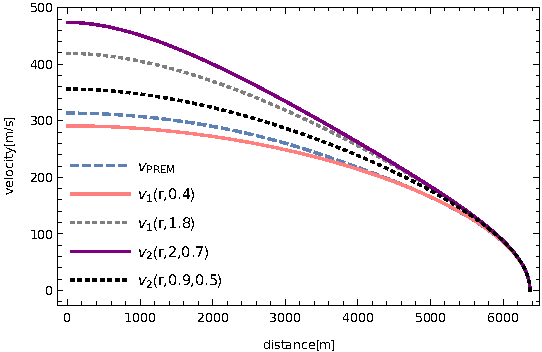
\includegraphics[scale=0.85]{Figures/some-velocities.pdf}
        \caption{Some velocity profiles of  the along with the numeric profile $v_{PREM}$.}
        \label{fig:some velocities}
    \end{figure}
    
    
    
\section{Traversal time}\label{time section}
        
    Sea $ds^2 = dr^2 + r^2 d\theta^2$ el intervalo infinitesimal de una trayectoria expresado en coordenadas polares, y $v(r)$ la velocidad instantánea de un objeto sobre esta trayectoria como funcion de $r$. El tiempo del trayecto viene dado por
            
            \begin{equation*}
                t = \int \frac{ds}{v(r)},
            \end{equation*}
    que de manera más conveniente se puede reescribir
            
            \begin{equation}
                t = \int \frac{\sqrt{r^2 + {r'}^2}}{v(r)} d\theta = \int \frac{\sqrt{ 1 + r^2 {\theta'}^2}}{v(r)} dr, 
                \label{tiempos}
            \end{equation}
    con ${r'} = dr/d\theta$ y $\theta' = d\theta / dr$. Cualquiera de las dos posibilidades de \eqref{tiempos} puede ser usada a conveniencia, según la descripción que se necesite para la trayectoria a considerar.
            
    \subsection{Traversal time between antipodes}
    
        Las antípodas son los dos puntos diametralmente opuestos en una esfera (los puntos más alejados entre sí), es decir, si el túnel gravitacional dentro de la Tierra se hace recto y pasando por el centro de la misma, se conectan las antípodas. Este camino es el más antiguamente considerado, y en el caso de la densidad constante da un tiempo de recorrido $T_0 = 42min$ \citep{History-Tunels}. También es el primero a considerar en toda la literatura sobre el tema por ser, claramente, el caso más sencillo. En la supocisión de gravedad constante se obtienen $T_{\text{const}} = 37min 58 s$, el desarrollo numérico de PREM da $T_{\text{prem}}=38min 11s$ \cite{gravity-train-prem}.  
        
        Siendo este último valor el que se desea obtener, seguimos a Iserman\citep{gravity-train-prem-approx} para definir las funciones a minimizar, de tal modo que los tiempos se acerquen a este valor
        
        \begin{align}
            f_1(b)=\int_0^1 \left( \frac{1}{\hat{v}_{prem}(x)}-\frac{1}{\hat{v}_1(x;b)} \right)^2 dx \label{f1 minimize}, \\
            f_2(b,c)=\int_0^1 \left( \frac{1}{\hat{v}_{prem}(x)}-\frac{1}{\hat{v}_2(x;b,c)} \right)^2 dx \label{f1 minimize},
        \end{align}
        siendo $\hat{v}$ las versiones adimencionales de las funciones consideradas en \eqref{perfil de v}. Usando un método apropiado y un lenguaje de programación avanzado (en nuestro caso usamos \emph{mathematica}), es fácil obtener
        
        \begin{align*}
            f_1: \{ b &\rightarrow 0.54 \} ,\\
            f_2: \{ b &\rightarrow 0.55 \; ,\; c \rightarrow 4.26 \}.
        \end{align*}
        
    Con estos valores en las funciones de densidad \eqref{densidad efectiva 1} y \eqref{densidad efectiva 2}, se puede obetener la gráfica de la figura \ref{fig:density}. Como se mencionó anteriormente, estas funciones, para los propósitos aquí considerados, no deben acertar en los valores de densidad correspondientes a cada capa interna, por lo que no supone ningún inconveniente que $\rho_2$ en el centro sea mayor a $\rho_{PREM}$, ni que las densidades en la superficie no sean exactamente las del agua. Si bien la motivación de este trabajo es meramente pedagógica, podría esperarse un uso astrofísico, mas no, claramente, geofísico.
    
    \begin{figure}
        \centering
        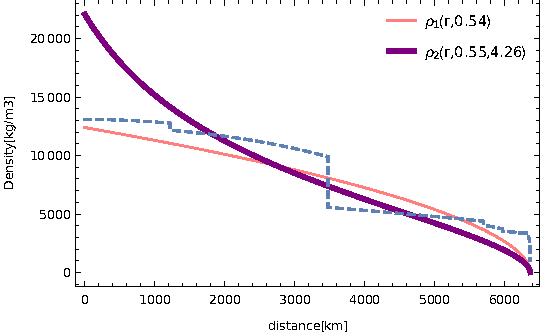
\includegraphics[scale=0.85]{Figures/densities.pdf}
        \caption{Effective density functions plotted along with numeric profile of PREM (dashed lines).}
        \label{fig:density}
    \end{figure}
    
    
    De manera análoga, usando ahora estos valores en los perfiles de velocidades, se puede observar una increíble coincidencia (ver figura  \ref{fig:velocity}). La velocidad máxima en las trayectorias antípodas predichas por cada función, son decentemente cercanas
    
    \begin{align*}
        v_{PREM}(0) &= 9915 m/s, \\
        v_1 (0,0.54)&= 9687 m/s ,\\
        v_2 (0,9.14,0.18) &=10001 m/s,
    \end{align*}
    mientras que los tiempos del trayecto completo, usando la parte derecha de \eqref{tiempos} con $\theta'=0$ y los perfiles de velocidad \eqref{velocidad efectiva 2} dan
    
    \begin{align*}
        T_{PREM} &= 38 \text{min} \hspace{0.1cm} 11.26 \text{s}, \\
        T_1 &= 38 \text{min}  \hspace{0.1cm} 05.7 \text{s},\\
        T_2 &= 38 \text{min} \hspace{0.1cm} 13.01 \text{s} ,
    \end{align*}
    lo que supone una discrepancia respecto al modelo de
    
    \begin{equation*}
        \Delta T_1 = 0.2\% \hspace{0.2cm}, \hspace{0.2cm}\Delta T_2 = 0.04. \%
    \end{equation*}
    
    \begin{figure}
        \centering
        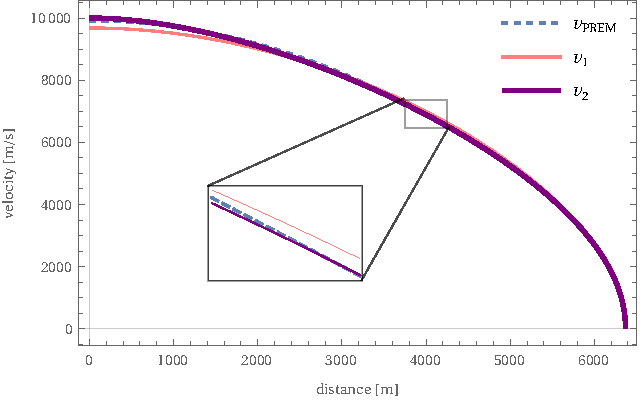
\includegraphics[scale=0.85]{Figures/velocities.pdf}
        \caption{Velocity profile of the model along with the ones obtained from the effective densities, for the path between antipodes.}
        \label{fig:velocity}
    \end{figure}
    
    Procedemos ahora a calcular los tiempos en otras trayectorias.
            
    \subsection{Chord Path}
    
        En términos de las distancia $d$, la más cercana de esta recta al centro de la esfera(ver figura \ref{fig:Earth drawing}) , la trayectoria se puede escribir a partir de las relaciones
            
        \begin{figure}
            \centering
            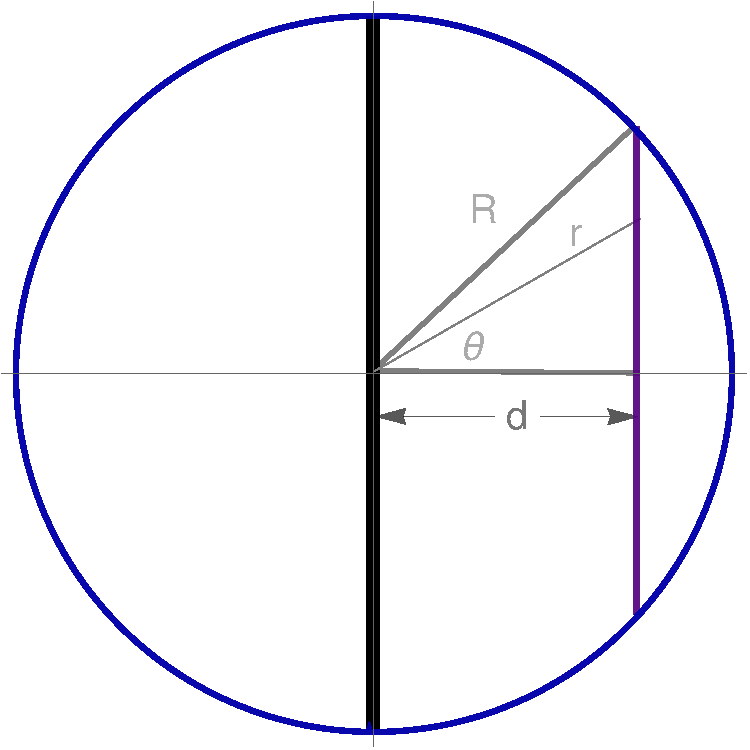
\includegraphics[scale=0.55]{Figures/earthdrawing.pdf}
            \caption{Representation of the Earth and the chord path at a distance $d$, with other useful parameters.}
            \label{fig:Earth drawing}
        \end{figure}    
            
        \begin{equation}
            r = \frac{d}{\cos{\theta}}
        \end{equation}
            
        con esto, la integral de la derecha en \eqref{tiempos} queda 
            
            \begin{equation*}
                t = \int \frac{r}{\sqrt{r^2 -d^2}} \frac{dr}{v(r)},
            \end{equation*}
            considerando ahora los límites, $r$ toma un máximo valor igual al radio de la esfera $R$, hasta un mínino valor $d$, para volver a llegar a $R$ en el otro extremo, por lo que los tiempos a resolver se hallan mediante
            
            \begin{equation}
                \frac{T}{2} =  \int_{d}^{R} \frac{r}{\sqrt{r^2 -d^2}} \frac{dr}{v(r)}.
                \label{tiempos camino recto}
            \end{equation}
            
            En la figura \ref{fig:times}, además de verse una increíble coincidencia entre ambas funciones resultado de la densidad efectiva y la proveniente del modelo, vemos la misma particularidad que se presenta en este tipo de trayectorias, independientemente del perfil de densidad, a saber, que los tiempos, de manera contraria a la intuición, son por pocos minutos mayores cuanto menor es la distancia.
            
            
            \begin{figure}
                \centering
                 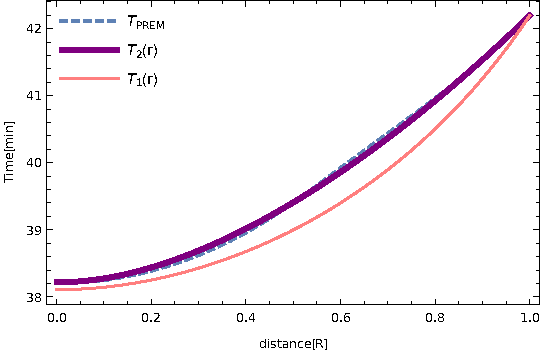
\includegraphics[scale=0.85]{Figures/times.pdf}
                \caption{Traversal time for the chord path between two arbitrary points on the surface as a function fo the distance $d$ of the path to the center of the Earth.}
                \label{fig:times}
            \end{figure}
            
            
\section{Braquistochrone Path}\label{braquistochrone section}
        
            La curva braquistócrona es por definición aquella en la cual el descenso o recorrido toma el menor tiempo, o del mismo modo, en el que las velocidades alcanzadas son mayores. Para hallar estas curvas,  como es usual, se usan métodos variacionales sobre  \eqref{tiempos} y se hallan las respectivas ecuaciones de Euler-Lagrange. Para ello tómese la integral a la izquierda, de modo que
            
            \begin{equation*}
                t = \int f(r, r', \theta) d\theta,
            \end{equation*}
            con
            
            \begin{equation}
                f= \frac{\sqrt{r^2 + (dr / d\theta )^2 } }{v(r)}, 
                \label{lagrangiano efectivo}
            \end{equation}
            que es mínima si se cumple
            
            \begin{equation}
               \frac{d}{d \theta } \left( \frac{\partial f}{\partial r'} \right)  - \frac{\partial f}{\partial r} = 0 ,
               \label{ec de Euler-Lagrange}
            \end{equation}
            y a partir de \eqref{ec de Euler-Lagrange} se pueden encontrar, integrando, las trayectorias $r=r(\theta)$. 
            
            Sin conocer la velocidad de manera explícita es posible desarrollar esta ecuación, usando regla de la cadena, y gracias a la no dependencia en $\theta$,
            
            \begin{equation*}
                r' \frac{\partial f}{\partial r'} - f = c ,
            \end{equation*}
            explícitamente
            
            \begin{equation*}
                \frac{1}{v(r)} \frac{{r'}^2}{\sqrt{{r'}^2 + r^2}} - \frac{\sqrt{{r'}^2 + r^2}}{v(r)} = c.
            \end{equation*}
            
            La constante se mantiene en cualquier momento de la trayectoria, en particular si $r \rightarrow r_{min} = d$, donde $r'=0$, de modo que
            
            \begin{equation*}
                c = -\frac{d}{v(d)},
            \end{equation*}
            por lo cual 
            
            \begin{equation*}
                 \frac{1}{v(r)} \frac{{r'}^2}{\sqrt{{r'}^2 + r^2}} - \frac{\sqrt{{r'}^2 + r^2}}{v(r)} =   -\frac{d}{v(d)},
            \end{equation*}
            y en general la ecuación de Euler-Lagrange es
            
            \begin{equation*}
                \frac{r^2}{\sqrt{{r'}^2 + r^2}} = d \frac{v(r)}{v(d)},
            \end{equation*}
            resolviendo para $r'$
            
            %\begin{equation*}
            %    {r'}^2 + r^2 = \frac{r^4 }{d^2} \left( \frac{v(d)}{v(r)} \right)^2
            %\end{equation*}
            
            %o 
            
            \begin{equation}
                r' = \left[ \frac{r^4 }{d^2} \left( \frac{v(d)}{v(r)} \right)^2 - r^2  \right]^{1/2} = g^{-1}(r),
                \label{función g de la trayectoria} 
            \end{equation}
            así, la trayectoria se puede hallar usando
            
            \begin{equation}
                \theta(r) = \int_{d}^{r} g(x) dx.
                \label{integral de la trayectoria}
            \end{equation}
    
    
            \begin{figure}
            \centering
            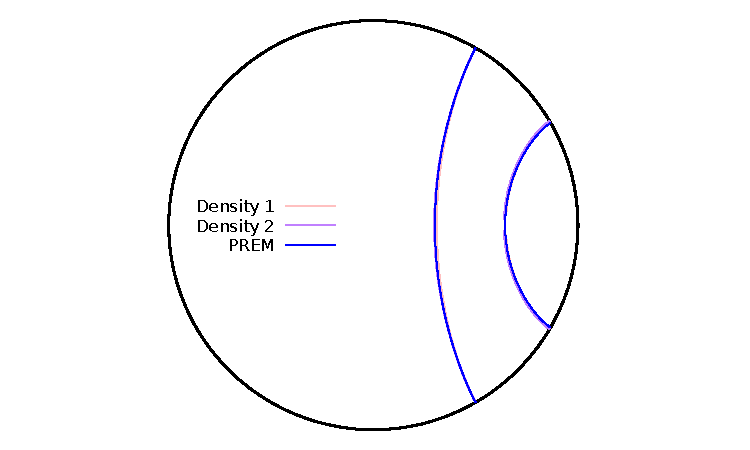
\includegraphics[scale=0.8]{Figures/brachistochrones.pdf}
            \caption{Shape of the brachistochrone curves for the PREM density and for the effective densities  \eqref{densidad efectiva 1} and \eqref{densidad efectiva 2}}
                \label{fig:braquistochrone}
            \end{figure}
    
        \subsection{Times for the brachistochrone path}
        
            Los tiempos para este camino pueden usarse nuevamente con \eqref{tiempos}, en este caso $\theta'$ se halla derivando \eqref{integral de la trayectoria} y  las mismas funciones de velocidad a considerar. Para los tres casos que trabajamos en este artículo, puede ver en la figura \ref{fig:braquistochrone times}. En cuanto a la cercanía que las funciones tienen unas con otras, es un buen indicio de que la física es la misma una vez se han fijado la aceleración de la gravedad en la superficie (o la masa), y los tiempos del camino más sencillo, y de que para el presente tratamiento es poco lo que se pierde al reemplaar el perfil numérico del modelo PREM por las densidades efectivas. En cuanto al comportamiento de estas tres funciones, que es el mismo para cualquier otra función densidad, los tiempos son menores si los caminos conectan puntos más cercanos sobre la superficie, lo cual es de esperar, además, los tiempos son para cualquier trayectoria con un acercamiento $d$ dado, siempre menores a los de los caminos rectos, salvo para el caso $d=0$ en el que la trayectorias, por supuesto, son las mismas y por tanto así sus tiempos de tunelamiento.
            
            
            \begin{figure}
                \centering
                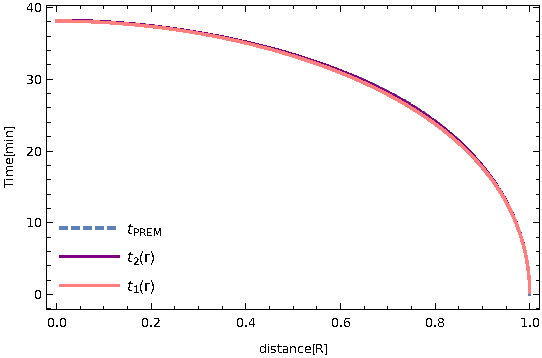
\includegraphics[scale=0.85]{Figures/braqtimes.pdf}
                \caption{Traversal time for the brachistochrone paths as a function of the minimum distance of the trayectory to the center of the Earth for each of the densities considered.}
                \label{fig:braquistochrone times}
            \end{figure}
            
            
        El por qué los tiempos de los caminos rectos es mayos si menor es el trayecto, y el porqué una braquistócrona, respecto a un camino recto, conectando los mismos dos puntos sobre la superficie toma un menor tiempo en recorrer siendo la longitud del túnel mayor, yace en la misma justificación a todo movimiento cinemático: la dinámica. Los resultados obtenidos para estos tiempos, que, como se mencionó, no son causa de la densidad sino de la forma misma de las trayectorias, cuando la densidad depende únicamente de la distancia al centro de la Tierra. Esto será discutido en la próxima sección.
        
\section{Acceleration}  \label{acceleration section}
    
        Poco es lo que se ha discutido en la literatura sobre la aceleración en la dirección de movimiento para cada trayectoria.
        Es verdad que todo el análisis, así como puede partir de una distribución de densidad dada, puede también hacerse desde un perfil de gravedad, y es de hecho así como se ha tomado en este y otros trabajos para la situación de la Tierra de acuerdo a PREM (dado que estos datos también fueron dados en el estudio original\cite{PREM}). No obstante, el caracter vectorial de esta aceleración también juega un papel crucial a la hora de entender qué camino tomará menos tiempo.
    
        En general, el valor de los tiempos se entiende como el resultado de una contraposición de la longitud de los caminos (cada vez menor) y la magnitud de las velocidades en cada punto (también cada vez menor), sin entender del todo por qué uno se sobrepone al otro en cada caso. Estudiar las aceleraciones y sus componente en la dirección del camino ayuda no solo a visualizar cuál de estas dos magnitudes favorece el valor del tiempo encontrado sino también da una explicación al por qué. 
   
        En últimas, lo que se hace es un análisis de la atracción gravitacional sobre un cuerpo de prueba de masa unidad, de manera que 
   
        \[ \Vec{F}_g (r) = \Vec{a}_r (r) ,\]
        estas aceleraciones ya se han calculado y aparecen en la figura \ref{fig:gravity}. Ahora, estas magnitudes corresponden al valor de la aceleración en dirección radial ($\hat{r}$). Para hallar la magnitud de estas aceleraciones en dirección de las trayectorias debe considerarse
        \[ a(r) = a_r \sin{\theta} ,\]
    
        para el caso de los caminos rectos corresponde a
    
        \[ a_{CHORD}(r) = a_r(r) \frac{\sqrt{r^2 - d^2}}{r}, \]
        mientras que para las trayectorias braquistócronas se usa el resultado hallado en \eqref{integral de la trayectoria}
        
        \[ a_{BRAQ}(r) = a_r(r) \sin{\left(\theta(r)\right)}. \]
        
        
        Estos resultados se encuentran graficados en la figura \ref{fig:a-chord and a-braq} partiendo únicamente de la aceleración $a_{r 1}$ en \eqref{aceleración gravitacional general}, en este punto se espera que el lector esté de acuerdo en que las gráficas para $a_{r PREM}$ y $a_{r 2}$ serán muy parecidas. Las seis curvas corresponden a $a_{CHORD}(r)$ en tres túneles rectos conectando diferentes puntos sobre la superficie (color rojo), y a $a_{BRAQ}$ para tres túneles que en principio conectan los mismos puntos sobre la superficie (color magenta), por esta razón ambos se encuentran en la superficie ($r/R=1$). Nótese además que la distancia de menor acercamiento $d$ es menor en las braquistócronas respecto a los caminos rectos, como se observa también en la forma de las trayectorias. Además, el valor de la aceleración en ese punto de menor acercamiento siempre es cero, dado que la tangente de la trayectoria siempre es perpendicular al radio.
        
        
        \begin{figure}
            \centering
            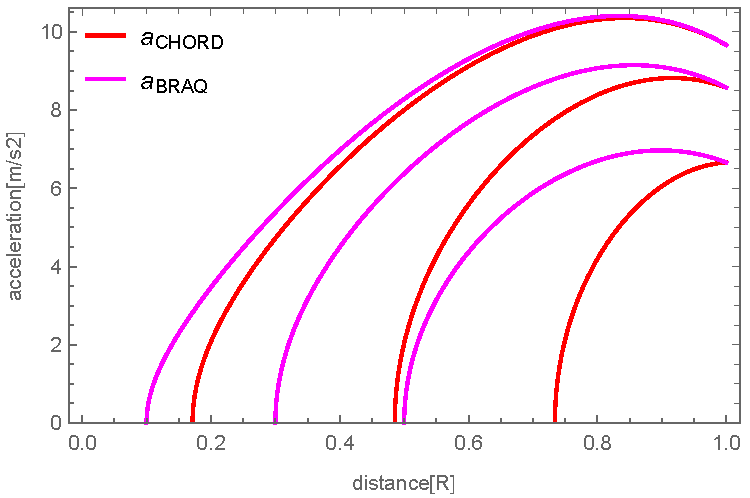
\includegraphics[scale=0.65]{Figures/acceleration.pdf}
            \caption{Acceleration in the direction of the movement for three chord paths (red online) and for three brachistochrone  paths (magenta online).}
            \label{fig:a-chord and a-braq}
        \end{figure}
        
        Respecto a los valores de las aceleraciones, que es lo que aquí nos concierne, hay que destacar dos puntos.
        
        \begin{itemize}
            \item Comparando las aceleraciones en la trayectoria recta, aquellas que corresponden a un menor $d$, es decir, que conectan dos puntos más alejados sobre la superficie y cuyo camino es más corto, se encuentran siempre por encima de las de menor $d$, es decir, para estos caminos la aceleración  es en todo punto de la trayectoria mayor que para caminos más cortos, y por lo tanto, sus velocidades son mayores, con lo cual, los tiempos son menores.
            
            \item El mismo comportamiento puede observarse entre las aceleraciones de las braquistócronas (en magenta) y las de los caminos rectos (en rojo). Las primeras se encuentran siempre por encima, lo que implica que sus velocidades en efecto son siempre mayores y lo tiempos, por consiguiente, menores.
            
        \end{itemize}
        
    \newline

\section{Conclusion}

    Como se ha mencionado, los modelos efectivos en física pueden llegar a tener un gran poder predictivo, a pesar de no estar describiendo la naturaleza real de los objetos. En el presente trabajo hemos encontrado, de manera exitosa, que los resultados de una función como ley de potencia decreciente se pueden ajustar muy acordemente a los obtenidos usando un modelo más descriptivo del interior de la Tierra, al abordar el problema del túnel gravitacional. Si bien la forma del perfil densidad o del perfil de aceleración no es el mejor ajuste a los del modelo numérico (ver fig. \ref{fig:density} y \ref{fig:gravity}), hay un gran acuerdo entre los perfiles de velocidades \ref{fig:velocity}. Los tiempos de tunelamiento en un túnel conectando antípodas, que para la situación de densidad constante es de $42 \text{min}$\cite{Venezian}, mientras que para una gravedad constante es de $37\text{min}$ \citep{gravity-train-prem}, han dado como resultado $38\text{min} 5 \text{s} $ para el caso de densidad con un parámetro (siendo el exponente $0.54$), y $38\text{min} 11.20 \text{s} $ para el caso de densidad con dos parámetros (siendo estos $9.14$ y $0.18$); respecto a los $38\text{min} 11.26 \text{s} $ que se encuentran con el conjunto de datos de PREM, por lo que nuestra función representa una descripción mucho más fiel a la Tierra que la primera aproximación de densidad constante, o que la aproximación de aceleración constante, que no dista mucho, a pesar de contener implicaciones físicas imposibles. 
    
    Adicional a ello se ha encontrado que los tiempos de tunelamiento de caminos rectos desplazados respecto al centro de la Tierra se superponen más para la densidad con dos parámetros que para la de un parámetro (ver fig. \ref{fig:times}), con respecto a los tiempos que realmente se obtendrían en el interior según PREM. Esto era de esperar, dado que las distribuciones de masa realmente son diferentes, pero aún así el acuerdo entre ambos es sorprendente. Lo mismo se mantiene para la forma de las braquistócronas (fig. \ref{fig:braquistochrone}) y los tiempos en los caminos de las braquistócronas (fig. \ref{fig:braquistochrone times}), en los que hay gran concordancia. Esto pareciera implicar que las funciones de densidad de masa encontradas no solo pueden dar cuenta de efectos exteriores, globales, sino también de ciertas características locales. Otra prueba de ello es que los perfiles de velocidad (fig. \ref{fig:velocity}) también se encuentran en completo acuerdo a lo largo de todas las distancias desde el centro hasta la superficie, y en en particular en el centro, donde se espera una menor coincidencia se encuentran discrepancias porcentuales del y $2.3\%$ para el perfil de densidad efectiva con un parámetro y del  $0.9\%$ para la función con dos parámetros.
    
    Cabe mencionar, no obstante, que la densidad efectiva que aquí proponemos pretende ser una simplificación matemática con el mismo contenido físico de la igualmente aproximación propuesta por PREM, y no una descripción de la Tierra misma. Factores como la rotación de la Tierra, irregularidades en las direcciones angulares o el hecho de que la Tierra no es una esfera no están tenidos en cuenta, sin embargo, la libertad en la escogencia de estos parámetros permitiría, en principio, extender la función de densidad de masa a otros planetas o cuerpos esféricos no muy densos ni masivos (dado que el perfil, como ha sido planteado, tampoco es capas de dar cuenta de efectos relativistas) y simular sus interiores mediante una relación matemática simple. Para ello habría que partir por el valor local de $\overline{\rho}$, fijar una constante de ``normalización'' de manera que la integración sobre todo el radio de la masa total correcta (o la gravedad en la superficie), y variar los parámetros a conveniencia. El primero de ellos; el exponente, altera como tal la forma y concavidad de la función, y es fácil ver que a mayor exponente se adquieren valores de densidad más altos en distancias más cercanas al centro. Esto quiere decir que densidades efectivas con mayores exponentes pueden describir objetos con mayor concentración de masa en el interior, para los que se obtienen tiempos menores; y contrariamente, funciones con exponentes más pequeños describirían cuerpos con distribuciones de masa más uniformes, contentiendo como límite $b=0$ el caso de densidad constante y un tiempo de tunelamiento máximo ($42 min$ con el $\overline{\rho}$ de la Tierra). En cuanto al parámetro $c$, su trabajo en la familia de funciones $Y_c =(1-c x)^b$ para un $b$ dado es moderar el valor de $Y$ en $1$ (que en nuestro caso es tomada como la superficie del planeta) sin cambiar el valor en $0$. Con esto, diferentes valores de $c$ (en el rango $[0,1]$) cambian la distribución de masa en regiones cercanas a la superficie. Nuevamente se obtiene como caso límite $c=0$ el caso de densidad constante y tiempo máximo, mientras que el límite $c=1$ nos resulta en la densidad efectiva de un parámetro donde la densidad en la superficie se anula y donde los tiempos de un determinado $b$ son mínimos. De esta manera puede verse que el jugar con estos dos parámetros puede describir distribuciones de densiad que den lugar a tiempos de tunelamientos desde tan solo unos minutos hasta un valor máximo en cada planeta.
    
    Ahora, lo anteriormente discutido es, al menos por ahora, solo una curiosidad. Faltará mucho para conocer lo suficientemente bien la densidad de otro cuerpo astronómico diferente a la Tierra para poder hacer un adecuado ajuste de parámetros, y quizá mucho más para encontrarle alguna utilidad al perfil de densidad efectivo en tales casos. No obstante, volviendo a la Tierra, de acuerdo a lo que se ha mensionado sobre el parámetro $c$ y su efecto en la función de densidad, podría proporcionársele un papel más importante en aplicaciones que se desempeñen más en regiones cercanas a la superficie, de manera que sean ciertos valores de densidad o de cantidades físicas derivadas en las capas externas, lo que se usen para fijar los valores en las funciones, y no los tiempos da caída del túnel gravitaciónal. 
    
    Para resumir, el trabajo aquí desarrollado es un primer acercamiento a una propuesta con posiblemente múltiples aplicaciones en el ámbito pedagógico e investigativo, no solo para la física sino para ciencias relacionadas con la Tierra u otros cuerpos celestes.
    
    
    


\begin{acknowledgments}

We gratefully acknowledge...

\end{acknowledgments}

% BEGIN While writing use BibTeX
\bibliography{AJPTemplate} % For BibTex
% END

%BEGIN For final version, copy and paste contents of .bbl file here after running BibTeX (note: biber does not work in this case.)

\begin{thebibliography}{10}

\bibitem{History-Tunels}, M. Selmke, "A note on the history of gravity tunnels," Am. J. Phys. 86, (2018)


\bibitem{Venezian}, G. Venezian, "Terrestrial Brachistochron," Am. J. Phys., 34, (1966)

\bibitem{Goldstein} H.Goldstein, C.P. Poole, and J.L. Safko, "Classical Mechanics," Chap 2. Variational Principles, Addison-Wesley (2000)

\bibitem{Tunel-friccioon} T. G. Concannon y G. Giordano, "Gravity tunnel drag," Online, \url{https://arxiv.org/pdf/1606.01852.pdf},  2016

\bibitem{Solomon2}, A. J. Solomon, " Sliding alond a Chord through a Rotating Earth,"  Math. Mag. , 113 (2006)

\bibitem{Iserman2} S. Iserman, "Free fall through the rotating and inhomogeneous Earth," Am. J. Phys. 87, 646 (2019)

\bibitem{Simonic} A. Simonic, "A note on a straight gravity tunnel through a rotating body," Am. J. Phys. 88, 499 (2020)

\bibitem{Taillet2018} R. Taillet, "Free falling inside flattened spheroids," Am. J. Phys. 86, 924 (2018)

\bibitem{Parker2017} E. Parker, "A relativistic gravity train," Gen. Relativ. Gravit.  49:106 (2017)

\bibitem{Seel} M. Sell, "The relativistic gravity train," Eur. J. Phys. 39, 3 (2018) 

\bibitem{Tunel-Potencia} W. D. Pesnell, "Flying through polytropes," Am. J. Phys., 84, (2016)    

\bibitem{Politropes2} A. Gjerl\o v, W. D. Pesnell "Orbits through polytropes," Am. J. Phys. 87, 452 (2019)    

\bibitem{gravity-train-prem} Alexander R. Klotz,"The gravity tunnel in a non-uniform Earth," Am. J. Phys. 83, (2015)

\bibitem{gravity-train-prem-approx} S. Iserman, "Analytical solution of gravity tunnels through an inhomogeneous Earth," Am. J. Phys. 87,(2019)
    
\bibitem{AstronomicalConstants} International Astronomical Union,  "Selected Astronomical Constants,"  in The Astronomical Almanac Online (2016)

\bibitem{Snyder1985} R. Snyder, "Twodensity model of the Earth," Am. J. Phys. 54, 511 (1986)

\bibitem{Dragoni2020} M. Dragoni, "Gravity in Earth’s Interior," Phys. Teach. 58, 97 (2020) 

\bibitem{PREM} Dziewonski, Adam M.; Anderson, Don L., "Preliminary reference Earth model," Physics of the Earth and Planetary Interiors,25, (1981)









    



\end{thebibliography}

\end{document}
